\documentclass{article}

\usepackage{amsmath}
\usepackage{graphicx}
\usepackage{enumitem}

\title{Hierophone Filter}
\author{Guy John \\ \texttt{guy@rumblesan.com}}

\begin{document}

\maketitle

\section{Introduction}
Analysis of the Hierophone filter, a basic three-pole low-pass filter built from three cascaded OTA based integrator cells.

\newpage

\subsection{Notations}

\begin{description}
\item $R_i$ is the value of the resistor through which the input signal is fed to the OTA
\item $R_s$ is the value of the resistor at the voltage divider input of the OTA
\item $R_f$ is the value of the resistor through which the integrator output is fed back to the OTA input
\item $C$ is the value of the integrators' capacitor
\item $v_{cv}$ is the cutoff frequency control voltage
\item $v_i(s)$ is the input voltage
\item $v_{out}(s)$ is the output voltage
\end{description}

\subsection{OTA Low-Pass Filter}

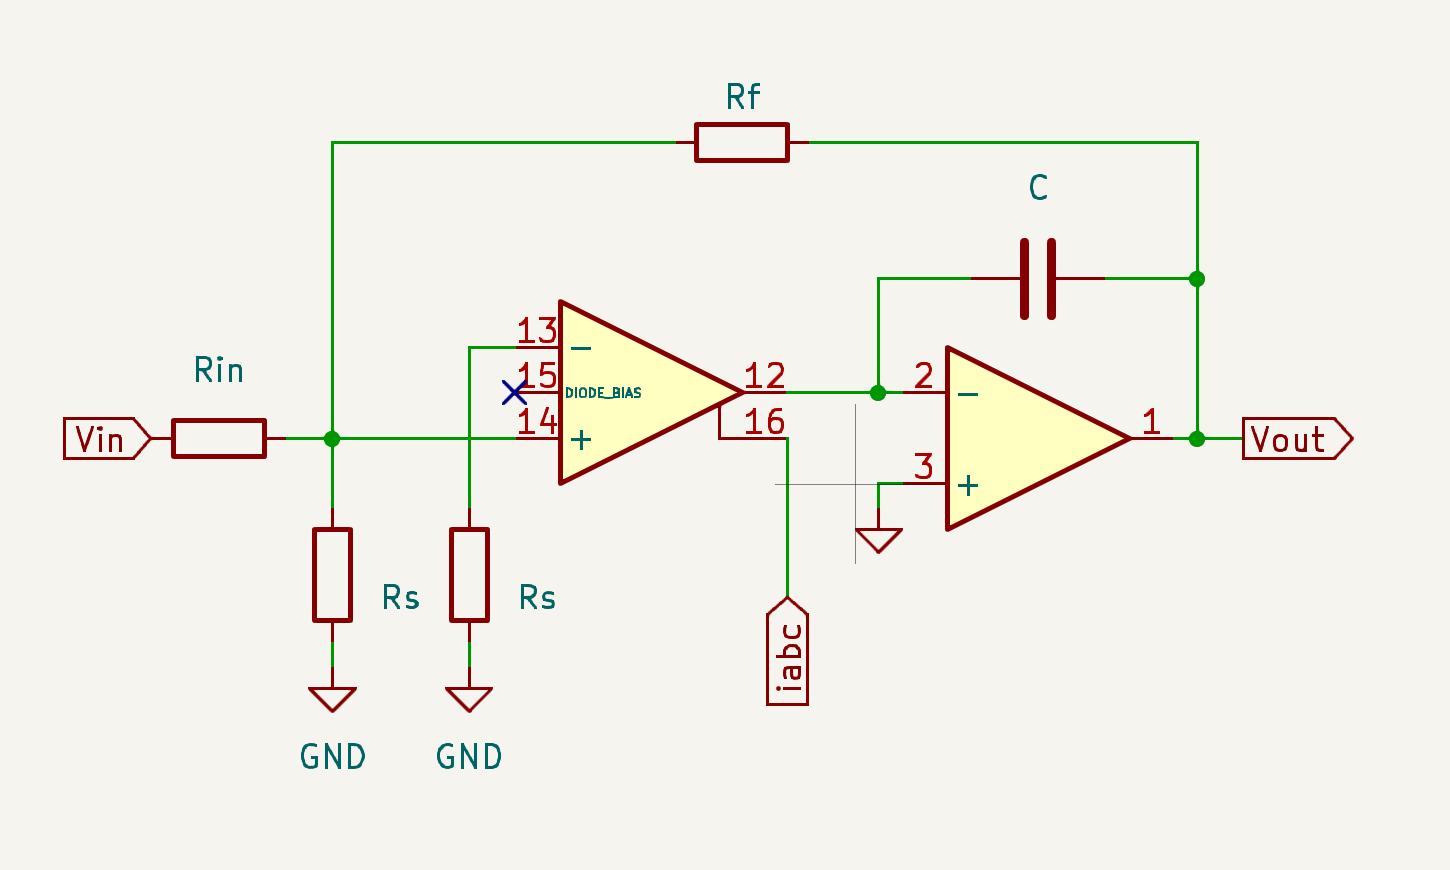
\includegraphics[width=\linewidth]{images/ota-low-pass.png}

The transfer function of an OTA is:

\begin{equation*}
\begin{split}
  i_o & = g_m(v_+ - v_-) \\
  i_o & = 19.2i_{cv}(v_+ - v_-) \\
\end{split}
\end{equation*}

If $R_f == R_i == R$ then Kirchoff in $v_+$ gives:

\begin{equation*}
\begin{split}
  \frac{1}{R}(v_i(s) - v_+(s)) + \frac{1}{R}(v_{out}(s) - v_+(s)) & = \frac{1}{R_s}v_+(s) \\
  v_+(s) & = \frac{R_s}{R + 2R_s}(v_i(s) + v_{out}(s)) \\
\end{split}
\end{equation*}

Given that $v_-$ is grounded, the current $i_c(s)$ at the output of the OTA is:

\begin{equation*}
\begin{split}
  i_c(s) & = g_m(v_+(s) - v_-(s)) \\
   & = 19.2i_{cv}\frac{R_s}{R + 2R_s}(v_i(s) + v_{out}(s)) \\
\end{split}
\end{equation*}

The voltage out of the OpAmp:

\begin{equation*}
\begin{split}
  v_{out}(s) & = \frac{-i_c(s)}{Cs} \\
  v_{out}(s) & = -19.2i_{cv}\frac{R_s}{Cs(R + 2R_s)}(v_i(s) + v_{out}(s)) \\
\end{split}
\end{equation*}

So the transfer function is:

\begin{equation}
  \alpha(s) = \frac{-1}{1 + \frac{R + 2 R_s}{R_s} Cs \frac{1}{19.2 i_{cv}}}
\end{equation}

The pole is at the frequency f so that:

\begin{equation*}
\begin{split}
  0 & = 1 + \frac{R + 2R_s}{R_s} C2\pi f \frac{1}{19.2 i_{cv}} \\
  f & = - \frac{19.2 i_{cv}}{2\pi\frac{R + 2 R_s}{R_s}C}\\
\end{split}
\end{equation*}

\subsection{Feedback Control}

The gain of the feedback circuit is:

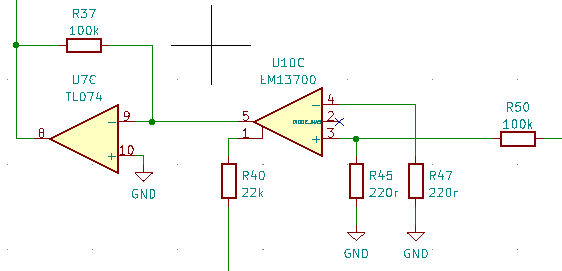
\includegraphics[width=\linewidth]{images/inverting-feedback-amp.png}

\begin{equation*}
\begin{split}
  v_+ & = v_i\frac{R_s}{R + R_s} \\
  i_o & = 19.2i_{q}(v_+ - v_-) \\
  i_o & = 19.2i_{q}(v_+ - 0) \\
  i_o & = 19.2i_{q}v_i\frac{R_s}{R + R_s} \\
  i_o & = R_f(v_- - v_o) \\
  i_o & = -R_fv_o \\
  -R_fv_o & = 19.2i_{q}v_i\frac{R_s}{R + R_s} \\
  -R_fv_o & = 19.2i_{q}v_i\frac{R_s}{R + R_s} \\
  v_o & = -19.2i_{q}v_i\frac{R_fR_s}{R_i + R_s} \\
  \beta & = -19.2i_{q}\frac{R_fR_s}{R_i + R_s} \\
\end{split}
\end{equation*}

\subsection{Filter}

\begin{equation*}
\begin{split}
  \frac{v_i - v_-}{R_i} + \frac{v_{hp} - v_-}{R_g} + \frac{v_{lp} - v_-}{R_g}  + \frac{v_{bp}\beta - v_-}{R_q} & = i_- = 0 \\
  \frac{v_i}{R_i} + \frac{v_{hp}}{R_g} + \frac{v_{lp}}{R_g}  + \frac{v_{bp}\beta}{R_q} & = 0 \\
\end{split}
\end{equation*}

It is important to note that $v_{bp}(s) = v_{hp}(s)\alpha(s)$, and $v_{lp}(s) = v_{hp}(s)\alpha(s^2)$.

\subsubsection{High-pass}

\begin{equation*}
\begin{split}
  \frac{v_{hp}(s)}{R_g} & = - \frac{v_i(s)}{R_i} - \frac{v_{lp}(s)}{R_g} - \frac{v_{bp}(s)\beta}{R_q} \\
  \frac{v_{hp}(s)}{R_g} & = - \frac{v_i(s)}{R_i} - \frac{v_{hp}(s)\alpha(s^2)}{R_g} - \frac{v_{hp}(s)\alpha(s)\beta}{R_q} \\
  \frac{v_i(s)}{R_i} & = - \frac{v_{hp}(s)}{R_g} - \frac{v_{hp}(s)\alpha(s^2)}{R_g} - \frac{v_{hp}(s)\alpha(s)\beta}{R_q} \\
  H_{hp}(s) & = \frac{v_{hp}(s)}{v_i(s)} \\
  \frac{v_i(s)}{R_i} & = - v_{hp}(s)(\frac{1}{R_g} + \frac{\alpha(s^2)}{R_g} + \frac{\alpha(s)\beta}{R_q}) \\
  \frac{1}{R_i} & = - H_{hp}(s)(\frac{1}{R_g} + \frac{\alpha(s^2)}{R_g} + \frac{\alpha(s)\beta}{R_q}) \\
  \frac{-1}{R_i} & = H_{hp}(s)(\frac{1}{R_g} + \frac{\alpha(s^2)}{R_g} + \frac{\alpha(s)\beta}{R_q}) \\
  H_{hp}(s) & = \frac{-1/R_i}{\frac{1}{R_g} + \frac{\alpha(s^2)}{R_g} + \frac{\alpha(s)\beta}{R_q}} \\
  & = \frac{-R_g/R_i}{1 + \frac{R_g\alpha(s)\beta}{R_q} + \alpha(s^2) } \\
\end{split}
\end{equation*}

\subsubsection{Low-Pass}

\begin{equation*}
\begin{split}
  H_{lp}(s) & = \frac{v_{lp}(s)}{v_i(s)} \\
            & = \frac{v_{hp}(s)}{v_i(s)}\alpha^2(s) \\
            & = \frac{-R_g/R_i}{\frac{1}{\alpha^2(s)} + \frac{R_g\beta}{R_q\alpha(s)} + 1 } \\
            & = \frac{-R_g/R_i}{\frac{1}{\alpha^2(s)} + \beta\frac{R_g}{R_q}\frac{1}{\alpha(s)} + 1 } \\
            & = \frac{-R_g/R_i}{\frac{1}{(-19.2i_{cv}\frac{R_s}{Cs(R + 2R_s)})^2} + (-19.2i_{q}\frac{R_fR_s}{R_i + R_s})\frac{R_g}{R_q}\frac{1}{-19.2i_{cv}\frac{R_s}{Cs(R + 2R_s)}} + 1 } \\
            & = \frac{-R_g/R_i}{\frac{1}{(19.2i_{cv}\frac{R_s}{Cs(R + 2R_s)})^2} + 19.2i_{q}\frac{R_fR_s}{R_i + R_s}\frac{R_g}{R_q}\frac{1}{19.2i_{cv}\frac{R_s}{Cs(R + 2R_s)}} + 1 } \\
            & = \frac{-R_g/R_i}{\frac{1}{\frac{1}{s^2}(19.2i_{cv}\frac{R_s}{C(R + 2R_s)})^2} + 19.2i_{q}\frac{R_fR_s}{R_i + R_s}\frac{R_g}{R_q}\frac{1}{19.2i_{cv}\frac{1}{s}\frac{R_s}{C(R + 2R_s)}} + 1 } \\
            & = \frac{-R_g/R_i}{\frac{s^2}{(19.2i_{cv}\frac{R_s}{C(R + 2R_s)})^2} + 19.2i_{q}\frac{R_fR_s}{R_i + R_s}\frac{R_g}{R_q}\frac{s}{19.2i_{cv}\frac{R_s}{C(R + 2R_s)}} + 1 } \\
\end{split}
\end{equation*}

One simplification worth making is to say that $R_q = R_g$.

By comparing with the standard form of a second order filter transfer function we can work out the following.

\begin{description}
  \item Pass-band gain, $-\frac{R_g}{R_i}$
  \item Cutoff frequency, $19.2i_{cv}\frac{R_s}{C2\pi(R + 2R_s)}$
  \item Quality factor, $\frac{1}{19.2i_{q}\frac{R_fR_s}{R_i + R_s}}$
\end{description}

\subsection{Calculating cutoff frequencies}

Given the calculation for frequency, and picking some standard values we can calculate cutoff for different $i_{cv}$ values.

\begin{description}
  \item $R$ is 100k
  \item $R_s$ is 220r
  \item $C$ is 220pF
\end{description}

\begin{equation}
  f = 19.2i_{cv}\frac{220}{220 * 10^{-12} * 2\pi(100000 + 2(220))}
\end{equation}

\begin{description}
  \item for $i_{cv}$ of 0.5ma $f = 15212Hz$
  \item for $i_{cv}$ of 0.3ma $f = 9127Hz$
  \item for $i_{cv}$ of 0.1ma $f = 3042Hz$
  \item for $i_{cv}$ of 0.05ma $f = 1521Hz$
  \item for $i_{cv}$ of 0.01ma $f = 304Hz$
\end{description}

\subsection{Calculating resonance}

A quality factor of $1/2$ gives no resonance, whilst the resonance (and likelihood of self oscillating) increases as Q goes to infinity.

\begin{description}
  \item $R_f$ is 100k
  \item $R_i$ is 100k
  \item $R_s$ is 220r
  \item $C$ is 220pF
\end{description}

\begin{equation}
  q = \frac{1}{19.2i_{q}\frac{100000 * 220}{100000 + 220}}
\end{equation}

\begin{description}
  \item for $i_{q}$ of 0.5ma $q = 0.47$
  \item for $i_{q}$ of 0.3ma $q = 0.79$
  \item for $i_{q}$ of 0.1ma $q = 2.37$
  \item for $i_{q}$ of 0.05ma $q = 4.75$
  \item for $i_{q}$ of 0.01ma $q = 23.7$
\end{description}


\end{document}
